\subsection{Measured implementation economy and unresolved timing}
\paragraph{Instruction-count confirmation.}
After native timing remained inconclusive, a bounded Callgrind 3.22.0 pass
compared the unchanged binaries on three specified cells. Counts at two batch
lengths subtract fixed command setup and diagnostic work. The resulting
per-repetition instruction slopes decrease in all three cases
(Table~\ref{tab:instructions}). Every profiled output retains the analytic
accuracy cap; baseline/candidate dense observations and counters also agree
within the profiler. Callgrind emulates instructions and may expose a different
SIMD feature set from native execution. Its instruction reduction is an actual
measured computational-work improvement, not a claim about native IPC or seconds.
The small fractional counts arise from differencing batch totals; small
serialization/control-path variation can remain in these estimates.

\begin{table}[t]
\caption{Measured Callgrind instruction slopes per solve/trajectory. Fixed
command costs are removed using two repetition lengths. All three changes
retain the same qualified numerical output in their profiled cohort.}
\label{tab:instructions}
\begin{ruledtabular}
\begin{tabular}{lrrr}
Scope & Baseline Ir & Candidate Ir & Reduction\\
\hline
lu $n=32$ & 13,489 & 11,709 & 13.196\% \\
dense $n=65$ & 59,721,066 & 58,165,078 & 2.605\% \\
adapter $n=16$ & 4,139,255 & 4,067,622 & 1.731\% \\
\end{tabular}
\end{ruledtabular}
\end{table}

\paragraph{Wall and process CPU timing.}
The first pass took 27.57 seconds. All eight active timing cohorts had paired
wall-time ranges spanning unity. The one-dimensional adapter case had correct,
identical trajectories but did not activate the new stop: its work remained
1644 units and its RHS count 1030 in both arms. It therefore received no
performance timing; this was not an accuracy failure.

Before further measurements, a single confirmation protocol selected four
diagnostic cells, increased baseline batches to approximately one second, and
added process user-plus-system CPU accounting. The confirmation took 99.17
seconds. No third timing pass was run. All four wall-time and process-CPU
block ranges still cross unity. In particular, the initially attractive
dimension-192 dense median of 1.252 reverses to 0.923 in the confirmation.
Reporting a reliable 25\% gain from the first pass would therefore be false.
The present environment supports the exact-work and allocation conclusions,
but does not resolve a stable wall-time benefit or regression for these paths.

\begin{table*}[t]
\caption{Long-batch confirmation. Each ratio is a median of five paired block
ratios. Ranges are observed minima/maxima, not confidence intervals. Process
CPU includes setup, diagnostic warmup and serialization; the adapter command
includes two initial diagnostic solves. Every range spans unity.}
\label{tab:confirmation}
\begin{ruledtabular}
\begin{tabular}{llrrrr}
Scope & $n$ & Wall ratio & Wall range & CPU ratio & CPU range\\
\hline
lu & 32 & 1.126 & 0.647--1.401 & 1.125 & 0.651--1.402 \\
dense & 65 & 1.033 & 0.626--1.202 & 1.028 & 0.629--1.214 \\
dense & 192 & 0.923 & 0.585--1.244 & 0.935 & 0.606--1.193 \\
adapter & 16 & 0.980 & 0.780--1.087 & 0.970 & 0.777--1.083 \\
\end{tabular}
\end{ruledtabular}
\end{table*}
\begin{figure*}[t]
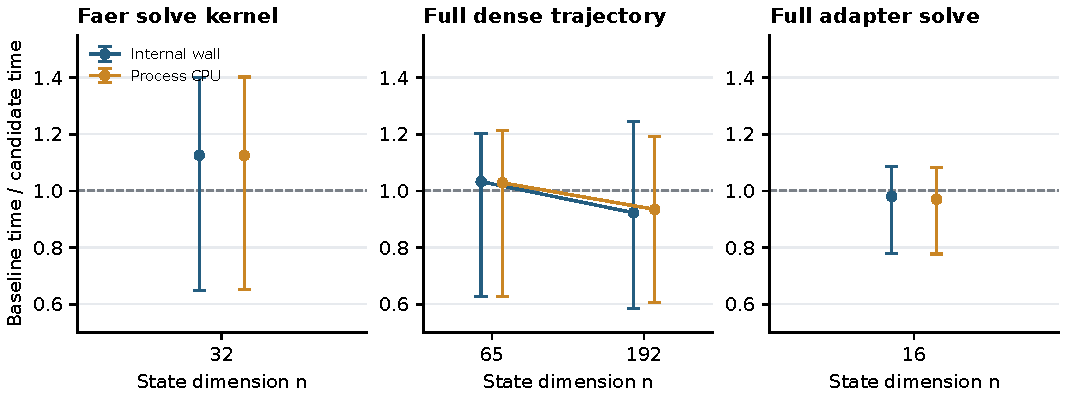
\includegraphics[width=\textwidth]{figures/performance.pdf}
\caption{Long-batch confirmation baseline/candidate time ratios. Points are medians of five
paired ABBA/BAAB block ratios; bars span the observed block minimum and maximum,
not a statistical confidence interval. Internal kernel wall time excludes
factorization. Full-solve wall intervals include setup, integration, output,
and counters. Process CPU additionally includes command warmup and serialization.
The adapter panel is a same-binary option comparison. All ranges cross unity.}
\label{fig:performance}
\end{figure*}
\begin{table*}[t]
\caption{Retained initial short-batch diagnostic timing. Values are median arm times;
speed ratios are medians of paired block ratios and need not equal the ratio
of the two displayed marginal medians. Every row passes its declared accuracy contract,
but none establishes a stable wall-time benefit.}
\label{tab:timing}
\begin{ruledtabular}
\begin{tabular}{llrrrrl}
Scope & $n$ & Baseline & Candidate & Ratio & Unit & Block-ratio range\\
\hline
LU solve & 32 & 2.128 & 1.598 & 1.074 & $\mu$s & 0.823--1.357 \\
LU solve & 96 & 10.524 & 10.357 & 1.078 & $\mu$s & 0.977--1.233 \\
LU solve & 192 & 14.895 & 14.901 & 0.996 & $\mu$s & 0.910--1.117 \\
Dense trajectory & 65 & 7.563 & 7.063 & 1.083 & ms & 0.928--1.248 \\
Dense trajectory & 96 & 16.999 & 16.960 & 1.022 & ms & 0.667--1.175 \\
Dense trajectory & 192 & 150.132 & 118.212 & 1.252 & ms & 0.844--1.598 \\
Adapter solve & 8 & 336.786 & 365.317 & 0.970 & $\mu$s & 0.859--1.099 \\
Adapter solve & 16 & 448.637 & 425.492 & 1.063 & $\mu$s & 0.945--1.095 \\
\end{tabular}
\end{ruledtabular}
\end{table*}
\begin{table}[b]
\caption{Dense trajectory accuracy on all 33 common times and all components.
All states, observation times, native counters and attempt counts are identical
in the baseline and candidate, with the same $10^{-7}$ error cap.}
\label{tab:dense-accuracy}
\begin{ruledtabular}
\begin{tabular}{lrl}
$n$ & Attempts & Maximum component error\\
\hline
65 & 81 & $4.595\times10^{-10}$ \\
96 & 81 & $4.617\times10^{-10}$ \\
192 & 81 & $4.605\times10^{-10}$ \\
\end{tabular}
\end{ruledtabular}
\end{table}
\begin{table*}[t]
\caption{Adapter work and accuracy. All accepted trajectory values are equal
between feature-off and feature-on runs. Every returned component, including
the common requested windows, meets the $10^{-5}$ cap. Work includes discarded
comparators; these reductions are not themselves time ratios.}
\label{tab:adapter-work}
\begin{ruledtabular}
\begin{tabular}{lrrrrrl}
$n$ & RHS off/on & Work off & Work on & Work reduction & Prefix wins & Maximum error\\
\hline
8 & 1120/1112 & 2119 & 2102 & 0.80\% & 1 & $6.101\times10^{-8}$ \\
16 & 1216/1200 & 2655 & 2605 & 1.88\% & 1 & $6.101\times10^{-8}$ \\
\end{tabular}
\end{ruledtabular}
\end{table*}
The sentinel-on control has identical complete trajectories and counters with
the new option off/on, as expected because the option does not change that path.
The targeted native contracts separately verify encountered-fatal priority,
conservative arithmetic near the exact-integer limit, and incomplete-evidence
semantics. The full raw records include rejected or failed build attempts as
well as successful validation. No broad historical test suite is relabeled
as a new execution.

\subsection{Negative and conditional theory results}
\begin{figure*}[t]
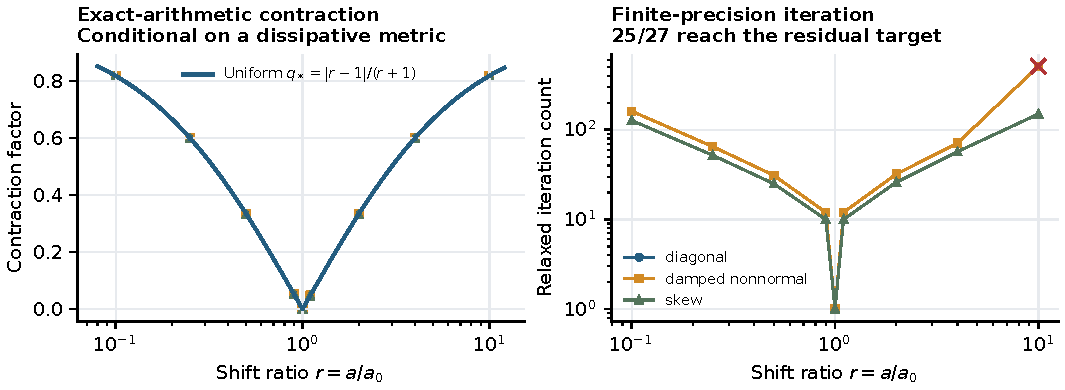
\includegraphics[width=\textwidth]{figures/theory.pdf}
\caption{Shifted-system research experiment. Left: the exact-arithmetic
uniform contraction bound and finite computed operator norms. Right: iteration
counts of the relaxed candidate. Red crosses mark two runs that reached the
512-iteration limit without attaining the unchanged $10^{-10}$ residual
threshold. Numeric norm checks are diagnostic checks, not interval certificates.}
\label{fig:theory}
\end{figure*}
\begin{table*}[t]
\caption{Selected shifted-system cells exposing both benefit and cost.
``Fail'' preserves the original stopping failure. Iteration counts are not
wall times and should not be compared as if their kernels had equal cost.}
\label{tab:theory-cells}
\begin{ruledtabular}
\begin{tabular}{llrrll}
Family & $a/a_0$ & Relaxed iterations & Unrelaxed iterations & Relaxed target & Unrelaxed target\\
\hline
diagonal & 0.1 & 161 & 44 & Pass & Fail \\
diagonal & 0.25 & 65 & 92 & Pass & Fail \\
diagonal & 4 & 71 & 61 & Pass & Pass \\
diagonal & 10 & 512 & 119 & Fail & Pass \\
damped nonnormal & 2 & 32 & 9 & Pass & Pass \\
damped nonnormal & 10 & 512 & 12 & Fail & Pass \\
skew & 1 & 1 & 1 & Pass & Pass \\
skew & 4 & 57 & 11 & Pass & Pass \\
\end{tabular}
\end{ruledtabular}
\end{table*}
The two failed relaxed residuals are approximately $4.80\times10^{-10}$ and
$4.67\times10^{-10}$, while their actual forward errors are small. This is
consistent with residual evaluation at a floating floor; it does not justify
changing the requested target after observing the failures. The new rule cures
two diagonal unrelaxed divergences but generally increases iterations elsewhere.
Consequently the theorem supplies a conditional convergence option, not an
unconditional performance replacement.
